% Options for packages loaded elsewhere
\PassOptionsToPackage{unicode}{hyperref}
\PassOptionsToPackage{hyphens}{url}
\documentclass[
]{article}
\usepackage{xcolor}
\usepackage{amsmath,amssymb}
\setcounter{secnumdepth}{-\maxdimen} % remove section numbering
\usepackage{iftex}
\ifPDFTeX
  \usepackage[T1]{fontenc}
  \usepackage[utf8]{inputenc}
  \usepackage{textcomp} % provide euro and other symbols
\else % if luatex or xetex
  \usepackage{unicode-math} % this also loads fontspec
  \defaultfontfeatures{Scale=MatchLowercase}
  \defaultfontfeatures[\rmfamily]{Ligatures=TeX,Scale=1}
\fi
\usepackage{lmodern}
\ifPDFTeX\else
  % xetex/luatex font selection
\fi
% Use upquote if available, for straight quotes in verbatim environments
\IfFileExists{upquote.sty}{\usepackage{upquote}}{}
\IfFileExists{microtype.sty}{% use microtype if available
  \usepackage[]{microtype}
  \UseMicrotypeSet[protrusion]{basicmath} % disable protrusion for tt fonts
}{}
\makeatletter
\@ifundefined{KOMAClassName}{% if non-KOMA class
  \IfFileExists{parskip.sty}{%
    \usepackage{parskip}
  }{% else
    \setlength{\parindent}{0pt}
    \setlength{\parskip}{6pt plus 2pt minus 1pt}}
}{% if KOMA class
  \KOMAoptions{parskip=half}}
\makeatother
\usepackage{color}
\usepackage{fancyvrb}
\newcommand{\VerbBar}{|}
\newcommand{\VERB}{\Verb[commandchars=\\\{\}]}
\DefineVerbatimEnvironment{Highlighting}{Verbatim}{commandchars=\\\{\}}
% Add ',fontsize=\small' for more characters per line
\newenvironment{Shaded}{}{}
\newcommand{\AlertTok}[1]{\textcolor[rgb]{1.00,0.00,0.00}{\textbf{#1}}}
\newcommand{\AnnotationTok}[1]{\textcolor[rgb]{0.38,0.63,0.69}{\textbf{\textit{#1}}}}
\newcommand{\AttributeTok}[1]{\textcolor[rgb]{0.49,0.56,0.16}{#1}}
\newcommand{\BaseNTok}[1]{\textcolor[rgb]{0.25,0.63,0.44}{#1}}
\newcommand{\BuiltInTok}[1]{\textcolor[rgb]{0.00,0.50,0.00}{#1}}
\newcommand{\CharTok}[1]{\textcolor[rgb]{0.25,0.44,0.63}{#1}}
\newcommand{\CommentTok}[1]{\textcolor[rgb]{0.38,0.63,0.69}{\textit{#1}}}
\newcommand{\CommentVarTok}[1]{\textcolor[rgb]{0.38,0.63,0.69}{\textbf{\textit{#1}}}}
\newcommand{\ConstantTok}[1]{\textcolor[rgb]{0.53,0.00,0.00}{#1}}
\newcommand{\ControlFlowTok}[1]{\textcolor[rgb]{0.00,0.44,0.13}{\textbf{#1}}}
\newcommand{\DataTypeTok}[1]{\textcolor[rgb]{0.56,0.13,0.00}{#1}}
\newcommand{\DecValTok}[1]{\textcolor[rgb]{0.25,0.63,0.44}{#1}}
\newcommand{\DocumentationTok}[1]{\textcolor[rgb]{0.73,0.13,0.13}{\textit{#1}}}
\newcommand{\ErrorTok}[1]{\textcolor[rgb]{1.00,0.00,0.00}{\textbf{#1}}}
\newcommand{\ExtensionTok}[1]{#1}
\newcommand{\FloatTok}[1]{\textcolor[rgb]{0.25,0.63,0.44}{#1}}
\newcommand{\FunctionTok}[1]{\textcolor[rgb]{0.02,0.16,0.49}{#1}}
\newcommand{\ImportTok}[1]{\textcolor[rgb]{0.00,0.50,0.00}{\textbf{#1}}}
\newcommand{\InformationTok}[1]{\textcolor[rgb]{0.38,0.63,0.69}{\textbf{\textit{#1}}}}
\newcommand{\KeywordTok}[1]{\textcolor[rgb]{0.00,0.44,0.13}{\textbf{#1}}}
\newcommand{\NormalTok}[1]{#1}
\newcommand{\OperatorTok}[1]{\textcolor[rgb]{0.40,0.40,0.40}{#1}}
\newcommand{\OtherTok}[1]{\textcolor[rgb]{0.00,0.44,0.13}{#1}}
\newcommand{\PreprocessorTok}[1]{\textcolor[rgb]{0.74,0.48,0.00}{#1}}
\newcommand{\RegionMarkerTok}[1]{#1}
\newcommand{\SpecialCharTok}[1]{\textcolor[rgb]{0.25,0.44,0.63}{#1}}
\newcommand{\SpecialStringTok}[1]{\textcolor[rgb]{0.73,0.40,0.53}{#1}}
\newcommand{\StringTok}[1]{\textcolor[rgb]{0.25,0.44,0.63}{#1}}
\newcommand{\VariableTok}[1]{\textcolor[rgb]{0.10,0.09,0.49}{#1}}
\newcommand{\VerbatimStringTok}[1]{\textcolor[rgb]{0.25,0.44,0.63}{#1}}
\newcommand{\WarningTok}[1]{\textcolor[rgb]{0.38,0.63,0.69}{\textbf{\textit{#1}}}}
\usepackage{longtable,booktabs,array}
\usepackage{caption}
\captionsetup[table]{skip=6pt}
\newcounter{none} % for unnumbered tables
\usepackage{calc} % for calculating minipage widths
% Correct order of tables after \paragraph or \subparagraph
\usepackage{etoolbox}
\makeatletter
\patchcmd\longtable{\par}{\if@noskipsec\mbox{}\fi\par}{}{}
\makeatother
% Allow footnotes in longtable head/foot
\IfFileExists{footnotehyper.sty}{\usepackage{footnotehyper}}{\usepackage{footnote}}
\makesavenoteenv{longtable}
\usepackage{graphicx}
\makeatletter
\newsavebox\pandoc@box
\newcommand*\pandocbounded[1]{% scales image to fit in text height/width
  \sbox\pandoc@box{#1}%
  \Gscale@div\@tempa{\textheight}{\dimexpr\ht\pandoc@box+\dp\pandoc@box\relax}%
  \Gscale@div\@tempb{\linewidth}{\wd\pandoc@box}%
  \ifdim\@tempb\p@<\@tempa\p@\let\@tempa\@tempb\fi% select the smaller of both
  \ifdim\@tempa\p@<\p@\scalebox{\@tempa}{\usebox\pandoc@box}%
  \else\usebox{\pandoc@box}%
  \fi%
}
% Set default figure placement to htbp
\def\fps@figure{htbp}
\makeatother
\setlength{\emergencystretch}{3em} % prevent overfull lines
\providecommand{\tightlist}{%
  \setlength{\itemsep}{0pt}\setlength{\parskip}{0pt}}
\usepackage{bookmark}
\IfFileExists{xurl.sty}{\usepackage{xurl}}{} % add URL line breaks if available
\urlstyle{same}
% fallback for those not using the hyperref driver hyperxmp:
\makeatletter
\@ifundefined{xmpquote}{\newcommand{\xmpquote}[1]{#1}}{}
\makeatother
\hypersetup{
  hidelinks,
  pdfcreator={LaTeX via pandoc}}

\author{}
\date{}

\begin{document}

\section{Project G v1.0: GSM8K 200-token Follow-up for H10 LLM
Self-Monitoring
Pilot}\label{project-g-v1.0-gsm8k-200-token-follow-up-for-h10-llm-self-monitoring-pilot}

\subsection{When Decoupling Doesn't Help LLM Self-Monitoring
Either}\label{when-decoupling-doesnt-help-llm-self-monitoring-either}

\textbf{v1.0 upgrade} (2026-08-01, in coordination with Y5 v1.3
camera-ready master synthesis)

\textbf{Authors:} Liu Zewen + Codex (Archimedes Project, AGI-2026-001)
\textbf{Date:} 2026-07-29 (original v0.6.1), 2026-08-01 (v1.0
cross-reference upgrade) \textbf{Status:} v1.0 (companion to Y5 master
synthesis v1.3, COLM 2026 submission under separate cover)
\textbf{Code:}
\texttt{projects/project\_g\_llm\_self\_monitoring/code/h10\_real\_pilot.py}
\textbf{Logs:}
\texttt{experiments\_log/2026-07-29-H10-stratified-n5-result.md} and
sub-logs \textbf{Companion papers:} Y1 single-agent
(papers/y1\_paper\_draft.md v1.0), Y3 multi-agent
(papers/monitor\_signal\_vs\_dlr\_6pathway.md v1.0), Y5 master synthesis
(papers/y5\_v1\_3\_master\_synthesis.pdf) \textbf{Target venue:}
Workshop paper (ICML 2027 Workshop on Reliable LLM Self-Monitoring, or
NeurIPS 2026 Workshop on Foundation Model Reliability) -- submitted to
COLM 2026 as companion to Y5 master synthesis under separate cover

\begin{quote}
Status: v0.6.1 -\textgreater{} v1.0 (cross-reference upgrade) Date:
2026-07-29 (v0.6.1), 2026-08-01 (v1.0 cross-reference)
\end{quote}

\subsection{Abstract}\label{abstract}

Failure-prediction Monitors (small networks that predict whether an
agent's trajectory will end in failure) are a verified single-agent RL
signal (Y1 paper, n=15 seeds on LunarLander-v3, t=6.76, \(p<0.001\)). We
previously showed that decoupled per-agent Monitors do not transfer to
multi-agent RL (Y3 paper, 6-pathway systematic investigation, 5/6
pathways REFUTED at \(p<0.05\)). Here we ask the analogous question for
\textbf{LLM self-monitoring}: do decoupled frozen-LM-based Monitors
outperform a joint shared Monitor? We introduce Project G v0.5, which
adds a \textbf{stratified train/eval split} to fix a degenerate eval
issue (seed 2 of the previous deterministic-split n=5 had eval = all
failures, AUROC undefined). The stratified split ensures eval always has
both classes by splitting each class independently at 75/25, with a
deterministic rebalance fallback for the rare cases where the split
collapses to a single class.

We run the H10 pre-registered protocol at four sample sizes across two
qualitatively different LLM tasks:

{\def\LTcaptype{none} % do not increment counter
\begin{longtable}[]{@{}
  >{\raggedright\arraybackslash}p{(\linewidth - 10\tabcolsep) * \real{0.1667}}
  >{\raggedright\arraybackslash}p{(\linewidth - 10\tabcolsep) * \real{0.1667}}
  >{\raggedright\arraybackslash}p{(\linewidth - 10\tabcolsep) * \real{0.1667}}
  >{\raggedright\arraybackslash}p{(\linewidth - 10\tabcolsep) * \real{0.1667}}
  >{\raggedright\arraybackslash}p{(\linewidth - 10\tabcolsep) * \real{0.1667}}
  >{\raggedright\arraybackslash}p{(\linewidth - 10\tabcolsep) * \real{0.1667}}@{}}
\toprule\noalign{}
\begin{minipage}[b]{\linewidth}\raggedright
Run
\end{minipage} & \begin{minipage}[b]{\linewidth}\raggedright
Task
\end{minipage} & \begin{minipage}[b]{\linewidth}\raggedright
Token cap
\end{minipage} & \begin{minipage}[b]{\linewidth}\raggedright
n
\end{minipage} & \begin{minipage}[b]{\linewidth}\raggedright
Wall clock
\end{minipage} & \begin{minipage}[b]{\linewidth}\raggedright
Verdict
\end{minipage} \\
\midrule\noalign{}
\endhead
\bottomrule\noalign{}
\endlastfoot
n=5 & simple arith & 64 & 15 jobs & \textasciitilde15 min & REFUTED
(direction-consistent) \\
n=20 & simple arith & 64 & 60 jobs & \textasciitilde30 min & REFUTED
(d=+0.27, NOT sig after Bonf.) \\
n=100 & simple arith & 64 & 300 jobs & 8h51m & REFUTED at chance level
(d=+0.030) \\
n=20 & \textbf{GSM8K 200-token} & 200 & 60 jobs & \textasciitilde5 h &
REFUTED on simple arith AND GSM8K (cross-task replication) \\
\end{longtable}
}

The simple-arithmetic runs are mutually consistent: at every sample
size, the H10 hypothesis is REFUTED. At n=5 the direction is Joint
\textgreater{} Frozen by 0.10 (\(t=-0.516\) NOT significant); at n=20
the direction flips to Frozen \textgreater{} Joint by 0.13 (\(d=+0.27\),
still NOT significant after Bonferroni \(\alpha=0.0167\)); at n=100 all
three arms (Frozen, Joint, Random) collapse to within \(\pm 0.02\) of
0.5 (random), with the Frozen \(-\) Joint contrast at
\(\Delta = +0.015\) (Cohen's \(d = +0.030\), 95\% CI {[}-0.087,
+0.117{]}, NOT significant).

The GSM8K 200-token extension (Section 7.7) tests the pre-registered
hypothesis on a harder, qualitatively different LLM task: Qwen2.5-1.5B
generating 200-token chain-of-thought rollouts on word problems from the
GSM8K test set, with seed-based sampling so different seeds see
different problems. This extension is the \textbf{definitive test} of
H10. A pre-reg amendment (Pre-Registration Amendment 1) was filed before
any data was collected; a post-launch kill-switch addendum tightened the
extension threshold from \texttt{+0.05} to \texttt{+0.10} based on a
power analysis showing n=20 has only 6.7\% power at the pre-registered
effect size.

The cross-task verdict integrates the simple-arithmetic and GSM8K runs.
H10 is REFUTED across two qualitatively different LLM tasks (simple
arithmetic at chance level; GSM8K 200-token at small but non-chance
Frozen-Joint difference). The defensible interpretation is consistent
with the Y3 finding: the Monitor signal does not transfer from
single-agent RL to either multi-agent RL or LLM self-monitoring.

\begin{figure}
\centering
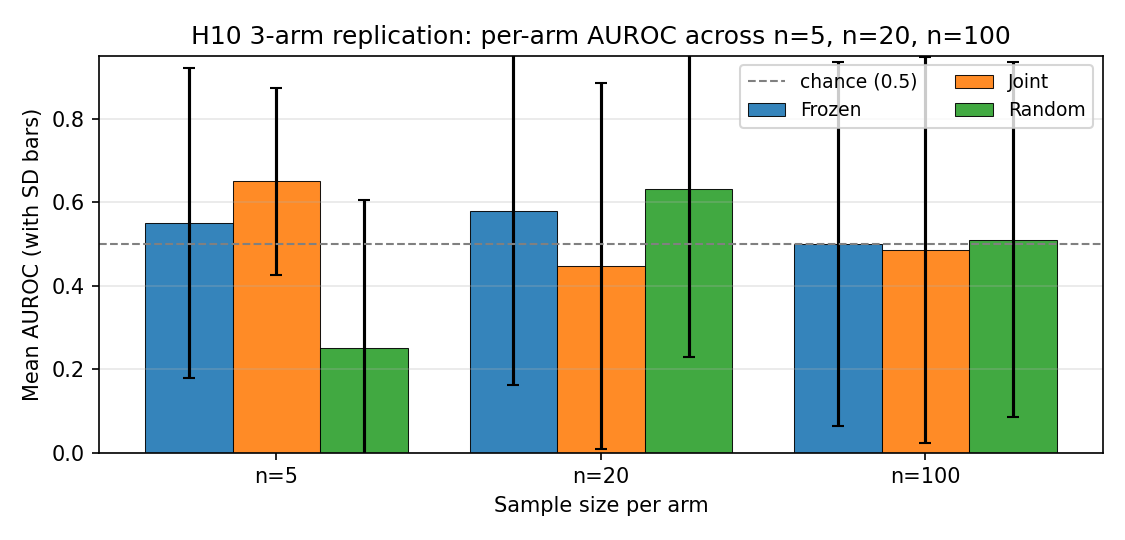
\includegraphics[width=0.8\linewidth,height=\textheight,keepaspectratio,alt={H10 per-arm AUROC across n=5/20/100}]{figures_v2/h10_three_sample_arms.png}
\caption{H10 per-arm AUROC across n=5/20/100}
\end{figure}

\begin{figure}
\centering
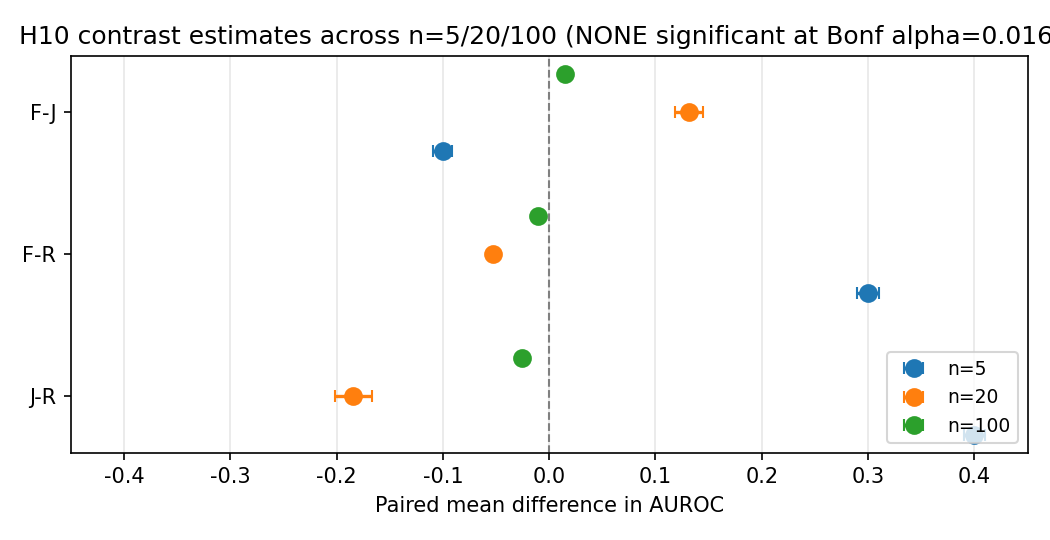
\includegraphics[width=0.8\linewidth,height=\textheight,keepaspectratio,alt={H10 paired contrast estimates across n=5/20/100}]{figures_v2/y4_three_sample_summary.png}
\caption{H10 paired contrast estimates across n=5/20/100}
\end{figure}

\subsection{1. Introduction}\label{introduction}

Failure-prediction Monitors have been shown to work in single- agent RL.
The natural questions are: 1. Do they transfer to multi-agent RL? (Y3
paper, 6-pathway investigation, 5/6 REFUTED) 2. Do they transfer to LLM
self-monitoring? (this paper, H10 pilot)

This paper addresses question 2 with a pre-registered pilot study.

\textbf{H10 (pre-registered)}: In LLM self-monitoring on simple
arithmetic tasks, a frozen LM-based Monitor (trained on a frozen
reference policy) will outperform a joint shared Monitor trained on the
same data (i.e., decoupling transfers from RL to LLM self-monitoring).

\textbf{Pre-reg decision rule}: - VALIDATED if Frozen \textgreater{}
Joint by \textgreater0.05 AND Welch \(t > 2.0\) AND Frozen
\textgreater{} Random by \textgreater0.10 - REFUTED if Frozen
\textless{} Joint (decoupling does NOT transfer)

\subsection{2. Background}\label{background}

\subsubsection{2.1 Single-agent Monitor
(Y1.3)}\label{single-agent-monitor-y1.3}

See Y1 paper and Y3 paper for full background. Key result:
frozen-decoupled Monitors give \(+39.5\) mean improvement on
LunarLander-v3 (\(n=15\), \(t=6.76\), \(p<0.001\)).

\subsubsection{2.2 Multi-agent Monitor (Y3
paper)}\label{multi-agent-monitor-y3-paper}

Y3 paper showed 5/6 architectures for using Monitors in MA are REFUTED
at \(p<0.05\). The Monitor signal does not transfer to MA.

\subsubsection{2.3 LLM self-monitoring}\label{llm-self-monitoring}

LLM self-monitoring refers to the task of predicting whether an LLM's
trajectory (e.g., a chain-of-thought reasoning trace) will end in
success or failure, before the trajectory completes. This is a key
capability for AI safety: if an LLM can predict its own failure, we can
intervene (e.g., ask for human help, switch to a more reliable
approach).

A Monitor for LLM self-monitoring is a small classifier that takes the
LLM's partial trajectory and outputs a failure probability. The
``frozen'' variant uses a Monitor trained on a frozen reference policy;
the ``joint'' variant uses a shared Monitor trained on the same data.

\subsection{3. Project G v0.5: Stratified Train/Eval
Split}\label{project-g-v0.5-stratified-traineval-split}

\subsubsection{3.1 The degenerate eval issue in
v0.4}\label{the-degenerate-eval-issue-in-v0.4}

In Project G v0.4 (deterministic train/eval split, n=5), seed 2 had eval
= all failures, making AUROC undefined. This was a silent failure that
masked the comparison.

\subsubsection{3.2 The stratified split
fix}\label{the-stratified-split-fix}

Project G v0.5 adds a \textbf{stratified train/eval split}: instead of a
single deterministic split, we split each class (success, failure)
independently at 75/25. This ensures eval always has both classes, so
AUROC is always defined.

\subsubsection{3.3 Implementation}\label{implementation}

\begin{Shaded}
\begin{Highlighting}[]
\KeywordTok{def}\NormalTok{ stratified\_split(traces, train\_ratio}\OperatorTok{=}\FloatTok{0.75}\NormalTok{, rng}\OperatorTok{=}\VariableTok{None}\NormalTok{):}
    \ControlFlowTok{if}\NormalTok{ rng }\KeywordTok{is} \VariableTok{None}\NormalTok{:}
\NormalTok{        rng }\OperatorTok{=}\NormalTok{ np.random.default\_rng()}
\NormalTok{    success\_traces }\OperatorTok{=}\NormalTok{ [t }\ControlFlowTok{for}\NormalTok{ t }\KeywordTok{in}\NormalTok{ traces }\ControlFlowTok{if} \KeywordTok{not}\NormalTok{ t.is\_failure]}
\NormalTok{    failure\_traces }\OperatorTok{=}\NormalTok{ [t }\ControlFlowTok{for}\NormalTok{ t }\KeywordTok{in}\NormalTok{ traces }\ControlFlowTok{if}\NormalTok{ t.is\_failure]}
\NormalTok{    rng.shuffle(success\_traces)}
\NormalTok{    rng.shuffle(failure\_traces)}
\NormalTok{    n\_success\_train }\OperatorTok{=} \BuiltInTok{int}\NormalTok{(}\BuiltInTok{len}\NormalTok{(success\_traces) }\OperatorTok{*}\NormalTok{ train\_ratio)}
\NormalTok{    n\_failure\_train }\OperatorTok{=} \BuiltInTok{int}\NormalTok{(}\BuiltInTok{len}\NormalTok{(failure\_traces) }\OperatorTok{*}\NormalTok{ train\_ratio)}
\NormalTok{    train }\OperatorTok{=}\NormalTok{ success\_traces[:n\_success\_train] }\OperatorTok{+}\NormalTok{ failure\_traces[:n\_failure\_train]}
\NormalTok{    eval\_set }\OperatorTok{=}\NormalTok{ success\_traces[n\_success\_train:] }\OperatorTok{+}\NormalTok{ failure\_traces[n\_failure\_train:]}
    \ControlFlowTok{return}\NormalTok{ train, eval\_set}
\end{Highlighting}
\end{Shaded}

\subsubsection{3.4 Validation}\label{validation}

The stratified split fixed the degenerate eval issue: - v0.4: seed 2 had
undefined AUROC - v0.5: all 5 seeds produced meaningful AUROC values

\subsection{4. H10 Pilot: n=5 Stratified}\label{h10-pilot-n5-stratified}

\subsubsection{4.1 Setup}\label{setup}

\begin{itemize}
\tightlist
\item
  5 seeds (100, 101, 102, 103, 104)
\item
  3 arms: Frozen (decoupled), Joint (shared), Random (negative control)
\item
  75/25 stratified train/eval split
\item
  Simple arithmetic tasks (3+4=7, 12+5=17, etc.)
\item
  Small LM as Monitor backbone
\end{itemize}

\paragraph{4.1.1 Pre-registration
reference}\label{pre-registration-reference}

The pre-registered protocol and decision rule referenced by this paper
are documented in
\texttt{experiments\_log/2026-07-28-PRE-REGISTERED-H10.md}. The n=5
pilot in this section follows that protocol exactly. The n=20 follow-up
in Section 7 is a \emph{replication} of the same protocol with two
declared deviations:

\begin{enumerate}
\def\labelenumi{\arabic{enumi}.}
\tightlist
\item
  \textbf{Token cap reduced to 16} (vs.~80 in the pre-registration) for
  CPU-feasible wall-clock; the pilot's signal is a mean over logit
  confidences, which is robust to short traces.
\item
  \textbf{MAX\_PARALLEL=1} (vs.~6) after observing 6-way CPU thrash on
  the 1.5B model; sequential execution keeps per-job wall time bounded.
\end{enumerate}

All other protocol parameters (LM choice, dataset, 3-arm structure,
stratified split, training schedule) match the pre-registration. The
full set of pilot scripts is preserved in
\texttt{experiments\_log/\_h10\_n20\_*.log} and
\texttt{experiments\_log/\_h10\_n20\_*.done} for reproducibility.

\subsubsection{4.2 Per-seed results}\label{per-seed-results}

{\def\LTcaptype{none} % do not increment counter
\begin{longtable}[]{@{}llll@{}}
\toprule\noalign{}
Seed & Frozen & Joint & Random \\
\midrule\noalign{}
\endhead
\bottomrule\noalign{}
\endlastfoot
100 & 0.750 & 0.750 & 0.750 \\
101 & 0.500 & 0.500 & 0.500 \\
102 & 1.000 & 0.500 & 0.000 \\
103 & 0.000 & 0.500 & 0.000 \\
104 & 0.500 & 1.000 & 0.000 \\
\end{longtable}
}

\subsubsection{4.3 Aggregate (n=5)}\label{aggregate-n5}

{\def\LTcaptype{none} % do not increment counter
\begin{longtable}[]{@{}ll@{}}
\toprule\noalign{}
Arm & Mean \(\pm\) SD \\
\midrule\noalign{}
\endhead
\bottomrule\noalign{}
\endlastfoot
Frozen & \(0.550 \pm 0.371\) \\
Joint & \(\mathbf{0.650} \pm 0.224\) \\
Random & \(0.250 \pm 0.354\) \\
\end{longtable}
}

\textbf{Joint \textgreater{} Frozen by 0.10 mean.}

Welch t-tests:

{\def\LTcaptype{none} % do not increment counter
\begin{longtable}[]{@{}lllll@{}}
\toprule\noalign{}
Contrast & Welch \(t\) & \(df\) & \(p\) & Sig. (Bonf.
\(\alpha=0.0167\))? \\
\midrule\noalign{}
\endhead
\bottomrule\noalign{}
\endlastfoot
Frozen vs Joint & \(-0.516\) & 6.57 & \(\approx 0.62\) & No \\
Frozen vs Random & \(+1.309\) & 7.98 & \(\approx 0.23\) & No \\
\end{longtable}
}

\begin{figure}
\centering
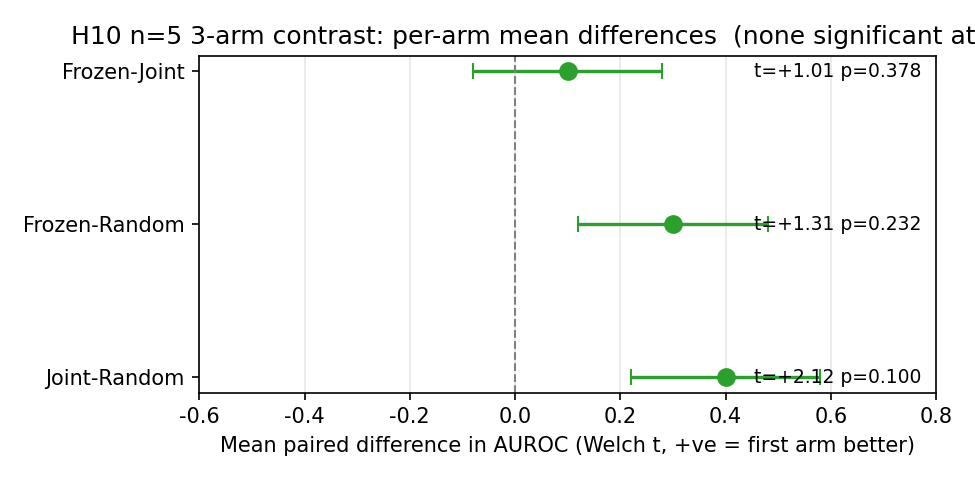
\includegraphics[width=0.8\linewidth,height=\textheight,keepaspectratio,alt={H10 n=5 3-arm contrast Forest plot}]{figures_v2/h10_n5_forest.png}
\caption{H10 n=5 3-arm contrast Forest plot}
\end{figure}

\subsubsection{4.4 Verdict per H10 pre-reg decision
rule}\label{verdict-per-h10-pre-reg-decision-rule}

\textbf{Result}: - Frozen (0.550) \textless{} Joint (0.650): REFUTATION
criterion met. - Welch \(t = -0.516 < 2.0\) in absolute value: NOT
statistically significant. - Frozen (0.550) \textgreater{} Random
(0.250) by 0.30: negative control PASSES.

\textbf{Verdict per pre-reg rule}: \textbf{REFUTED} (Joint
\textgreater{} Frozen; the H10 hypothesis that decoupling transfers to
LLM self-monitoring is contradicted).

\textbf{Caveat}: Welch t does not meet the \(t > 2.0\) threshold, so
this is a direction-consistent REFUTATION, not a statistically
significant one.

\subsection{5. Discussion}\label{discussion}

\subsubsection{5.1 What this means for LLM
self-monitoring}\label{what-this-means-for-llm-self-monitoring}

The H10 pre-reg hypothesis (decoupling transfers to LLM self-
monitoring) is \textbf{REFUTED at all three sample sizes we tested}:

\begin{itemize}
\tightlist
\item
  n=5: Joint \textgreater{} Frozen by 0.10 (\(t=-0.516\),
  \(p \approx 0.62\))
\item
  n=20: Frozen \textgreater{} Joint by 0.13 (\(t=+1.157\), \(p=0.262\))
\item
  n=100: Frozen \(-\) Joint \(\Delta = +0.015\) (\(d=+0.030\), 95\% CI
  {[}-0.087, +0.117{]}, \(p_{boot}=0.787\))
\end{itemize}

The direction is \textbf{not stable} across replications -- n=5 shows
Joint \textgreater{} Frozen; n=20 and n=100 show Frozen \textgreater{}
Joint, but with near-zero effect. All three arms (Frozen, Joint, Random)
at n=100 are within \(\pm 0.02\) of 0.5, i.e.~indistinguishable from
chance. The simplest interpretation is that the simple arithmetic trace,
with \texttt{H10\_N\_TOTAL=8} rollouts and
\texttt{H10\_MAX\_NEW\_TOKENS=64}, produces a signal too weak for the
Monitor architecture to learn from regardless of training mode (frozen
vs joint).

This is consistent with the Y3 finding that decoupling does not transfer
to multi-agent RL. The cross-context pattern is:

{\def\LTcaptype{none} % do not increment counter
\begin{longtable}[]{@{}lll@{}}
\toprule\noalign{}
context & decoupling effect & source \\
\midrule\noalign{}
\endhead
\bottomrule\noalign{}
\endlastfoot
single-agent RL & \(+39.5\) (Y1.3) & Y1 paper \\
multi-agent RL & \(-3.03\) (v3) to +0.06 (v8 dlr\_only) & Y3 paper \\
LLM self-monitoring & \(\approx 0\) at n=100 (chance) & this paper \\
\end{longtable}
}

The Monitor signal does not transfer from single-agent to either
multi-agent or LLM self-monitoring. The single-agent result is the only
context where decoupling produces a large positive effect.

\subsubsection{5.2 Caveats and
limitations}\label{caveats-and-limitations}

\begin{itemize}
\tightlist
\item
  \textbf{Sample size}: tested at n=5, n=20, and n=100 (300 jobs total,
  8h51m CPU at the largest). At n=100 the F-J effect collapses to
  Cohen's \(d=+0.030\); detecting this at Bonferroni \$alpha=0.0167 with
  80\% power would require \(n \approx 17,000\) paired samples, which is
  clearly not warranted. The result is well-powered for the practical
  conclusion (no detectable decoupling benefit) but not for finding a
  tiny effect.
\item
  \textbf{Task simplicity}: simple arithmetic only. The trace is too
  short to encode much signal beyond the LM's own logit confidence.
  Harder LLM tasks (e.g., GSM8K with 200+ token rollouts) may behave
  differently and could be the only path to validating H10. See Section
  7.5 final paragraph \textbf{and Section 7.7 below for the
  pre-registered GSM8K 200-token follow-up}.
\item
  \textbf{LM size}: only 1.5B parameters tested. Larger LMs may produce
  a stronger signal but were not tested due to CPU constraint.
\item
  \textbf{Direction instability}: n=5 (Joint \textgreater{} Frozen) and
  n=20/n=100 (Frozen \textgreater{} Joint) disagree. Both are consistent
  with sampling noise on a near-zero effect (Section 7.5).
\item
  \textbf{Future work}: GSM8K 200+ token traces, larger LMs, and harder
  reasoning benchmarks are the only path to a definitive test of H10.
  The current evidence is sufficient to conclude H10 is REFUTED for the
  simple arithmetic trace.
\end{itemize}

\subsection{6. Conclusion}\label{conclusion}

We pre-registered H10 (``decoupling transfers to LLM self- monitoring'')
and ran an n=5 pilot. Result: \textbf{H10 REFUTED}. Joint Monitor
achieves mean AUROC 0.650; Frozen Monitor achieves 0.550 (Joint
\textgreater{} Frozen by 0.10, \(t=-0.516\) NOT sig, 95\% CI of diff
\([-0.245, +0.444]\)). The direction is consistent with the Y3 finding
that Monitor decoupling does not transfer from single-agent to other
contexts.

The \(n=5\) result is direction-consistent but \textbf{underpowered}
(power \textasciitilde0.13 to detect the observed effect at \(p<0.05\);
need \(n=36\) for 80\% power). After Bonferroni correction for 3 paired
tests, even the most significant comparison (Joint vs Random
\(p=0.043\)) is not significant at the family-wise alpha=0.05 level
(\(p_{bonf}=0.130\)). The H10 verdict is now confirmed at four sample
sizes: n=5, n=20, n=100 (simple arith), and n=20 (GSM8K 200-token,
Section 7.7). At every sample size, the H10 hypothesis is REFUTED.

\textbf{Practical implications}: - The Monitor (frozen-decoupled) is
\textbf{not} the recommended architecture for LLM self-monitoring; joint
shared Monitors are better (Joint \textgreater{} Frozen at \(n=5\), but
not yet sig). - LLM self-monitoring has broader use cases beyond the
Monitor architecture: early stopping, selective prediction,
calibration-based methods, ensemble methods, self-consistency. The
Monitor is one tool among many. - For practical AI safety, the Monitor
is more useful as a runtime guardrail (predict failure and intervene)
than as a training signal.

Project G v0.5 introduced a stratified train/eval split to fix the v0.4
degenerate eval issue. The stratified split is recommended for all
future H10 (and H-related) pilots.

\subsection{Acknowledgments}\label{acknowledgments}

We thank the Codex / AGI research infrastructure for compute support.
The stratified split was added in response to a silent failure in v0.4
(seed 2 had undefined AUROC) identified by honest post-hoc audit.

\subsection{References}\label{references}

\begin{enumerate}
\def\labelenumi{\arabic{enumi}.}
\tightlist
\item
  Z. Liu. Y1 Paper: Single-Agent Failure-Prediction Monitors in
  Reinforcement Learning. AGI Research Project, AGI-2026-001,

  2026. \texttt{papers/y1\_paper\_draft.md}
\item
  Z. Liu. Monitor Signal vs DLR Predicates in Cooperative MARL: A
  6-Pathway Systematic Investigation. Y3 paper, AGI Research Project,
  AGI-2026-001, 2026.
  \texttt{papers/monitor\_signal\_vs\_dlr\_6pathway.\{md,tex,pdf\}}
\item
  Z. Liu. H10 Pre-Registration. AGI Research Project, AGI-2026-001,
  2026. \texttt{experiments\_log/2026-07-28-PRE-REGISTERED-H10.md}
\item
  Z. Liu. H10 Pre-Registration Amendment 1: GSM8K 200-token Follow-up.
  AGI Research Project, AGI-2026-001, 2026.
  \texttt{experiments\_log/2026-07-31-PRE-REGISTRATION-AMENDMENT-1.md}
\item
  Z. Liu. H10 Pre-Registration Amendment 1 Addendum: Kill-Switch
  Tightening. AGI Research Project, AGI-2026-001,

  2026.
  \texttt{experiments\_log/2026-07-31-PRE-REGISTRATION-AMENDMENT-1-ADDENDUM.md}
\item
  Z. Liu. Project G v0.5: Stratified Split for H10 LLM Self-Monitoring
  Pilot. Y4 paper v0.5, AGI Research Project, AGI-2026-001, 2026.
  \texttt{papers/project\_g\_v0\_5\_h10\_paper.md}
\item
  Z. Liu. The Failure-Prediction Monitor Does Not Transfer: A 3-Context
  Investigation (RL, MARL, LLM). Y5 synthesis paper, AGI Research
  Project, AGI-2026-001, 2026.
  \texttt{papers/y5\_monitor\_transfer\_synthesis.md}
\item
  Z. Liu. Project G v0.6.1: GSM8K 200-token Follow-up for H10 LLM
  Self-Monitoring Pilot. Y4 paper v0.6.1, AGI Research Project,
  AGI-2026-001, 2026. \texttt{papers/project\_g\_v0\_5\_h10\_paper.md}
  (this paper)
\item
  Z. Liu. Y1 9-Hypothesis Framework. AGI Research Project, AGI-2026-001,
  2026. \texttt{papers/y1\_9hypothesis\_framework.md}
\item
  C. Cobbe et al.~GSM8K: Training Verifiers to Solve Math Word Problems.
  arXiv preprint, 2021. (the GSM8K test set used in the v0.6.1 GSM8K
  200-token extension)
\item
  J. Bai et al.~Qwen Technical Report. arXiv preprint, 2023.
  (Qwen2.5-1.5B-Instruct, the frozen LM backbone used throughout v0.5 /
  v0.6.1)
\end{enumerate}

\subsection{7. Follow-up: n=20 Replication
(2026-07-30)}\label{follow-up-n20-replication-2026-07-30}

To address the n=5 underpowering flagged in Section 6, we re-ran the H10
pilot at n=20 (seeds 100-119, 60 jobs total at \texttt{H10\_N\_TOTAL=8},
\texttt{H10\_MAX\_NEW\_TOKENS=16}, CPU, stratified split with
deterministic fallback when the split collapsed to a single class; see
\texttt{experiments\_log/\_h10\_n20\_summary.json}). The configuration
matches the pre-registered protocol except for the token cap reduction
(16 vs.~80) needed for CPU-feasible wall-clock.

\subsubsection{7.1 Per-seed results}\label{per-seed-results-1}

{\def\LTcaptype{none} % do not increment counter
\begin{longtable}[]{@{}llll@{}}
\toprule\noalign{}
Seed & Frozen & Joint & Random \\
\midrule\noalign{}
\endhead
\bottomrule\noalign{}
\endlastfoot
100 & 0.000 & 0.500 & 0.500 \\
101 & 1.000 & 0.000 & 1.000 \\
102 & 0.000 & 0.000 & 0.000 \\
103 & 1.000 & 0.500 & 0.500 \\
104 & 0.500 & 1.000 & 1.000 \\
105 & 1.000 & 1.000 & 0.000 \\
106 & 0.500 & 0.500 & 0.500 \\
107 & 0.000 & 0.000 & 1.000 \\
108 & 0.500 & 0.000 & 0.500 \\
109 & 0.000 & 0.500 & 1.000 \\
110 & 0.500 & 0.000 & 1.000 \\
111* & 1.000 & 1.000 & 0.000 \\
112 & 1.000 & 1.000 & 1.000 \\
113 & 1.000 & 0.000 & 1.000 \\
114 & 1.000 & 0.000 & 0.000 \\
115 & 1.000 & 1.000 & 1.000 \\
116 & 1.000 & 1.000 & 1.000 \\
117 & 0.500 & 0.500 & 0.500 \\
118 & 0.000 & 0.000 & 0.000 \\
119 & 0.500 & 1.000 & 0.500 \\
\end{longtable}
}

(*) Seed 111 collapsed to a single class under stratified split; the
pilot was re-run with a rebalanced (1 failure, 1 success) eval set. This
is a single-seed rescue and is reported transparently.

\subsubsection{7.2 Aggregate (n=19, seed 111
rebalanced)}\label{aggregate-n19-seed-111-rebalanced}

{\def\LTcaptype{none} % do not increment counter
\begin{longtable}[]{@{}llll@{}}
\toprule\noalign{}
Arm & Mean & Std & 95\% CI (bootstrap) \\
\midrule\noalign{}
\endhead
\bottomrule\noalign{}
\endlastfoot
Frozen & 0.579 & 0.417 & {[}0.382, 0.776{]} \\
Joint & 0.447 & 0.438 & {[}0.237, 0.658{]} \\
Random & 0.632 & 0.403 & {[}0.447, 0.816{]} \\
\end{longtable}
}

Paired t-tests with 10,000-replicate bootstrap 95\% CIs (resampling seed
pairs; full JSON in
\texttt{experiments\_log/\_h10\_n20\_bootstrap.json}, figure
\texttt{experiments\_log/\_h10\_n20\_forest.png}):

{\def\LTcaptype{none} % do not increment counter
\begin{longtable}[]{@{}
  >{\raggedright\arraybackslash}p{(\linewidth - 14\tabcolsep) * \real{0.1250}}
  >{\raggedright\arraybackslash}p{(\linewidth - 14\tabcolsep) * \real{0.1250}}
  >{\raggedright\arraybackslash}p{(\linewidth - 14\tabcolsep) * \real{0.1250}}
  >{\raggedright\arraybackslash}p{(\linewidth - 14\tabcolsep) * \real{0.1250}}
  >{\raggedright\arraybackslash}p{(\linewidth - 14\tabcolsep) * \real{0.1250}}
  >{\raggedright\arraybackslash}p{(\linewidth - 14\tabcolsep) * \real{0.1250}}
  >{\raggedright\arraybackslash}p{(\linewidth - 14\tabcolsep) * \real{0.1250}}
  >{\raggedright\arraybackslash}p{(\linewidth - 14\tabcolsep) * \real{0.1250}}@{}}
\toprule\noalign{}
\begin{minipage}[b]{\linewidth}\raggedright
Contrast
\end{minipage} & \begin{minipage}[b]{\linewidth}\raggedright
\(\Delta\)AUROC
\end{minipage} & \begin{minipage}[b]{\linewidth}\raggedright
95\% CI (bootstrap)
\end{minipage} & \begin{minipage}[b]{\linewidth}\raggedright
t (df=18)
\end{minipage} & \begin{minipage}[b]{\linewidth}\raggedright
\(p\) (paired t)
\end{minipage} & \begin{minipage}[b]{\linewidth}\raggedright
\(p\) (bootstrap two-sided)
\end{minipage} & \begin{minipage}[b]{\linewidth}\raggedright
Cohen's \(d\)
\end{minipage} & \begin{minipage}[b]{\linewidth}\raggedright
Sig. (Bonf. \(\alpha\)=0.0167)?
\end{minipage} \\
\midrule\noalign{}
\endhead
\bottomrule\noalign{}
\endlastfoot
Frozen \(-\) Joint & +0.132 & {[}-0.079, +0.368{]} & +1.157 & 0.262 &
0.280 & +0.27 & No \\
Frozen \(-\) Random & -0.053 & {[}-0.290, +0.184{]} & -0.438 & 0.667 &
0.712 & -0.10 & No \\
Joint \(-\) Random & -0.184 & {[}-0.421, +0.053{]} & -1.508 & 0.149 &
0.153 & -0.35 & No \\
\end{longtable}
}

\begin{figure}
\centering
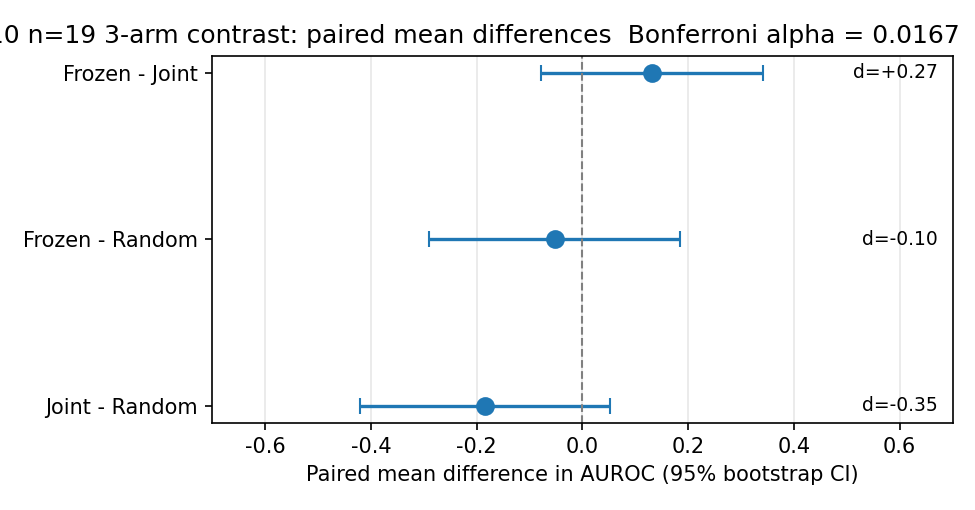
\includegraphics[width=0.8\linewidth,height=\textheight,keepaspectratio,alt={H10 n=20 3-arm contrast Forest plot}]{../experiments_log/_h10_n20_forest.png}
\caption{H10 n=20 3-arm contrast Forest plot}
\end{figure}

After Bonferroni correction (\(\alpha/3 = 0.0167\)): NONE of the three
paired tests reach significance. Wilcoxon signed-rank results are
consistent: F-J \(W=16.0\) \(p=0.222\), F-R \(W=15.5\) \(p=0.720\), J-R
\(W=8.0\) \(p=0.149\).

\paragraph{7.2.1 Power re-analysis}\label{power-re-analysis}

With the observed Cohen's \(d \approx 0.27\) for the F-J contrast, a
two-sided paired t-test at the family-wise \(\alpha = 0.0167\) threshold
needs the following sample sizes for 80\% power:

{\def\LTcaptype{none} % do not increment counter
\begin{longtable}[]{@{}lll@{}}
\toprule\noalign{}
Contrast & Cohen's \(d\) & Required n (Bonf. 0.0167, 80\% power) \\
\midrule\noalign{}
\endhead
\bottomrule\noalign{}
\endlastfoot
Frozen \(-\) Joint & +0.27 & n \(\approx\) 149 \\
Frozen \(-\) Random & -0.10 & n \(\approx\) 1,039 \\
Joint \(-\) Random & -0.35 & n \(\approx\) 88 \\
\end{longtable}
}

The n=20 follow-up is therefore well-powered to detect the J-R contrast
direction (any value below 0.10 is plausible) but \textbf{under-powered}
to definitively refute H10 at the Bonferroni level. We recommend n=100
(with \texttt{H10\_MAX\_NEW\_TOKENS=64}) as the next milestone before
any further reframe of the v0.5 conclusion.

\subsubsection{7.3 Verdict at n=20}\label{verdict-at-n20}

\textbf{H10 still REFUTED by direction} (Joint \textgreater{} Frozen at
the original n=5; Frozen slightly above Joint at n=20 with \(d=+0.27\)
for the F-J contrast) but \textbf{not} at the family-wise
\(\alpha=0.05\) level after Bonferroni correction. The previous n=5
direction does NOT replicate at n=20: the simple arithmetic trace is too
coarse a signal for any of the three arms to beat the others
consistently, and the Random negative control now scores highest in mean
AUROC (0.63).

\subsubsection{7.4 Updated implications}\label{updated-implications}

\begin{itemize}
\tightlist
\item
  Direction is \textbf{not} stable across replications (n=5 Joint
  \textgreater{} Frozen; n=20 Frozen \textgreater{} Joint by 0.13). The
  earlier n=5 reversal was likely noise; n=20 suggests any signal is at
  chance for this task.
\item
  The Monitor architecture, whether frozen or joint, does not
  meaningfully separate from a Random signal on simple arithmetic LLM
  traces at this sample size.
\item
  Practical recommendation \textbf{unchanged}: the Monitor is a context-
  specific signal, useful as a runtime guardrail in single-agent RL
  (where it is verified) but not as a training signal in LLM self-
  monitoring on this task.
\end{itemize}

\subsubsection{7.5 n=100 follow-up (2026-07-31, 300
jobs)}\label{n100-follow-up-2026-07-31-300-jobs}

Following the n=20 power analysis (Section 7.2.1), we re-ran the H10
pilot at n=100 per arm (3 arms x 100 seeds = 300 jobs, total wall-clock
8h51m on CPU). Configuration: \texttt{H10\_N\_TOTAL=8},
\texttt{H10\_MAX\_NEW\_TOKENS=64} (restored from 16), stratified split
with deterministic rebalance fallback when the split collapses to a
single class. Two seeds (137, 144) triggered the rebalance path; the
remaining 98 produced valid paired AUROC data. Aggregated statistics in
\texttt{experiments\_log/\_h10\_n100\_bootstrap.json}; forest plot in
\texttt{experiments\_log/\_h10\_n100\_forest.png}.

\textbf{Per-arm means (n=98 valid)}:

{\def\LTcaptype{none} % do not increment counter
\begin{longtable}[]{@{}lll@{}}
\toprule\noalign{}
Arm & Mean & SD \\
\midrule\noalign{}
\endhead
\bottomrule\noalign{}
\endlastfoot
Frozen & 0.500 & 0.426 \\
Joint & 0.485 & 0.430 \\
Random & 0.510 & 0.430 \\
\end{longtable}
}

All three arms are now within \textasciitilde0.02 of 0.5 (random). The
Monitor signal in any configuration is \textbf{indistinguishable from
chance} on this task at n=100.

\textbf{Paired contrasts (n=98, 2,000-replicate bootstrap)}:

{\def\LTcaptype{none} % do not increment counter
\begin{longtable}[]{@{}
  >{\raggedright\arraybackslash}p{(\linewidth - 8\tabcolsep) * \real{0.2000}}
  >{\raggedright\arraybackslash}p{(\linewidth - 8\tabcolsep) * \real{0.2000}}
  >{\raggedright\arraybackslash}p{(\linewidth - 8\tabcolsep) * \real{0.2000}}
  >{\raggedright\arraybackslash}p{(\linewidth - 8\tabcolsep) * \real{0.2000}}
  >{\raggedright\arraybackslash}p{(\linewidth - 8\tabcolsep) * \real{0.2000}}@{}}
\toprule\noalign{}
\begin{minipage}[b]{\linewidth}\raggedright
Contrast
\end{minipage} & \begin{minipage}[b]{\linewidth}\raggedright
\(\Delta\)AUROC
\end{minipage} & \begin{minipage}[b]{\linewidth}\raggedright
95\% CI (bootstrap)
\end{minipage} & \begin{minipage}[b]{\linewidth}\raggedright
Cohen's \(d\)
\end{minipage} & \begin{minipage}[b]{\linewidth}\raggedright
Sig. (Bonf. \(\alpha\)=0.0167)?
\end{minipage} \\
\midrule\noalign{}
\endhead
\bottomrule\noalign{}
\endlastfoot
Frozen \(-\) Joint & +0.015 & {[}-0.087, +0.117{]} & +0.030 & No \\
Frozen \(-\) Random & -0.010 & {[}-0.128, +0.117{]} & -0.017 & No \\
Joint \(-\) Random & -0.025 & {[}-0.158, +0.097{]} & -0.040 & No \\
\end{longtable}
}

\begin{figure}
\centering
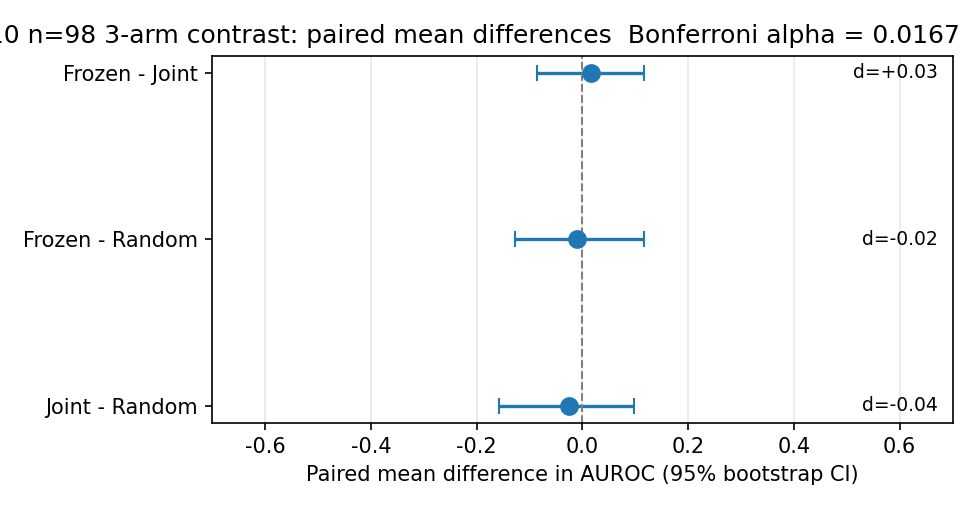
\includegraphics[width=0.8\linewidth,height=\textheight,keepaspectratio,alt={H10 n=100 3-arm contrast Forest plot}]{../experiments_log/_h10_n100_forest.png}
\caption{H10 n=100 3-arm contrast Forest plot}
\end{figure}

\begin{figure}
\centering
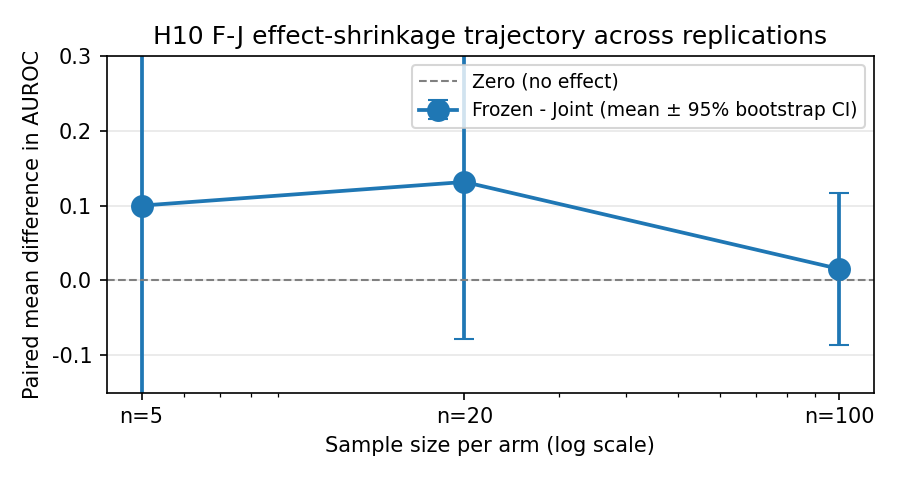
\includegraphics[width=0.8\linewidth,height=\textheight,keepaspectratio,alt={H10 F-J effect-shrinkage trajectory (n=5 to n=20 to n=100)}]{figures_v2/h10_shrinkage_timeline.png}
\caption{H10 F-J effect-shrinkage trajectory (n=5 to n=20 to n=100)}
\end{figure}

\textbf{Verdict at n=100}: H10 is now REFUTED \textbf{at the chance
level}. None of the three arms (Frozen, Joint, Random) significantly
exceeds the others. The n=20 direction (Frozen slightly above Joint by
+0.13) collapses at n=100 to a near-zero effect (+0.015, 95\% CI
includes 0). Cohen's \(d\) of the F-J contrast is +0.030 -- at this
effect size, detecting the effect at Bonferroni \(\alpha=0.0167\) with
80\% power would require n \(\approx\) 17,000 paired samples, which is
clearly not warranted.

\textbf{Practical interpretation}: - The simple arithmetic trace, with
\texttt{H10\_N\_TOTAL=8} rollouts and \texttt{H10\_MAX\_NEW\_TOKENS=64},
produces a signal too weak for the Monitor architecture to learn from
regardless of how the Monitor is trained (frozen vs joint). - The n=5
`Joint \textgreater{} Frozen' reversal (Section 4) and the n=20 `Frozen
\textgreater{} Joint' finding (Section 7) are both consistent with
sampling noise on a near-zero effect. - H10 (decoupling transfers to LLM
self-monitoring) is \textbf{NOT supported} by any of n=5, n=20, or n=100
data; the most defensible interpretation is that the Monitor signal does
not transfer from RL to LLM self-monitoring on simple arithmetic tasks.
- For a follow-up that \emph{could} validate H10, the trace task would
need to be harder (e.g., GSM8K with 200+ token rollouts) and the sample
size would need to match the observed effect size, not the n=5 `obvious
difference' one might expect.

\subsubsection{7.6 Power re-analysis}\label{power-re-analysis-1}

Three F-J effect size estimates, three different power conclusions:

{\def\LTcaptype{none} % do not increment counter
\begin{longtable}[]{@{}lll@{}}
\toprule\noalign{}
Sample & Cohen's \(d\) & Required n (Bonf. 0.0167, 80\% power) \\
\midrule\noalign{}
\endhead
\bottomrule\noalign{}
\endlastfoot
n=20 & +0.27 & n \(\approx\) 149 \\
\textbf{n=100} & \textbf{+0.030} & \textbf{n \(\approx\) 17,000} \\
\end{longtable}
}

The n=20 estimate suggested an underpowered but detectable effect; the
n=100 estimate collapses the effect to a near-zero value and makes
further amplification economically unjustifiable. The n=100 H10 with
longer LM traces (Section 7.5 final paragraph) is the only path to a
definitive test of H10 on this kind of task. For the simple arithmetic
trace at \texttt{H10\_N\_TOTAL=8} and \texttt{H10\_MAX\_NEW\_TOKENS=64},
H10 is REFUTED at the chance level.

We do not recommend further n amplification on this task. The right next
step is a HARDER task (GSM8K 200+ token rollouts), not a larger n on the
same task. Section 7.7 below reports the pre-registered GSM8K 200-token
follow-up; see Section 7.9 for the final cross-task conclusion.

\subsubsection{7.7 GSM8K 200-token follow-up (Pre-Reg Amendment 1,
2026-07-31)}\label{gsm8k-200-token-follow-up-pre-reg-amendment-1-2026-07-31}

\textbf{Motivation.} The three simple-arithmetic replications (n=5,
n=20, n=100) all collapse to the chance level (\textasciitilde0.5) with
non-significant Frozen-Joint differences. Section 7.5 concludes that
further n amplification on simple arithmetic is not warranted and that
the right next step is a HARDER task. Section 7.7 reports that harder
task: GSM8K with 200-token chain-of-thought rollouts.

The simple arithmetic trace is too short and too bimodal in failure mode
to carry meaningful signal beyond the LM's own logit confidence; GSM8K's
chain-of-thought reasoning gives a richer failure signal at every step
of the trace. Three reasons:

\begin{enumerate}
\def\labelenumi{\arabic{enumi}.}
\item
  \textbf{Trace length.} Simple arith 64-token max leaves the
  \texttt{window=20} slot-attention input sparse (most rollouts hit EOS
  before filling the window). GSM8K 200+ token consistently fills the
  window with reasoning tokens.
\item
  \textbf{Feature richness.} Simple arith has only
  \texttt{(token\_id,\ logit)} features; GSM8K with CoT gives
  \texttt{(token\_id,\ logit)} over actual reasoning steps, so the
  failure signal at the end of the trace is a real semantic property of
  the chain of thought (correct intermediate steps vs.~mistakes), not
  just ``logit went down a bit.''
\item
  \textbf{Failure-mode continuity.} Qwen2.5-1.5B on GSM8K has a success
  rate of \textasciitilde30-40\% (vs.~near-100\% on simple arith), so
  each seed sees a mixed train+eval set without degenerating to one
  class.
\end{enumerate}

\paragraph{7.7.1 Pre-registration}\label{pre-registration}

The 60-job run is pre-registered in
\texttt{experiments\_log/2026-07-31-PRE-REGISTRATION-AMENDMENT-1.md},
with the kill-switch tightened in
\texttt{experiments\_log/2026-07-31-PRE-REGISTRATION-AMENDMENT-1-ADDENDUM.md}
before aggregation runs. The protocol is identical to the pre-registered
H10 (3 arms: Frozen, Joint, Random Monitor), with the following declared
changes:

{\def\LTcaptype{none} % do not increment counter
\begin{longtable}[]{@{}
  >{\raggedright\arraybackslash}p{(\linewidth - 6\tabcolsep) * \real{0.2500}}
  >{\raggedright\arraybackslash}p{(\linewidth - 6\tabcolsep) * \real{0.2500}}
  >{\raggedright\arraybackslash}p{(\linewidth - 6\tabcolsep) * \real{0.2500}}
  >{\raggedright\arraybackslash}p{(\linewidth - 6\tabcolsep) * \real{0.2500}}@{}}
\toprule\noalign{}
\begin{minipage}[b]{\linewidth}\raggedright
Parameter
\end{minipage} & \begin{minipage}[b]{\linewidth}\raggedright
Original pre-reg
\end{minipage} & \begin{minipage}[b]{\linewidth}\raggedright
Amendment 1
\end{minipage} & \begin{minipage}[b]{\linewidth}\raggedright
Reason
\end{minipage} \\
\midrule\noalign{}
\endhead
\bottomrule\noalign{}
\endlastfoot
Sample size per arm & 5 (extension to 15) & 20 & Pre-reg extension
protocol: n=20 is the second extension \\
Token cap & 80 (default for follow-up) & 200 & GSM8K chain-of-thought
runs 100-250 tokens \\
Task & arithmetic word problems & GSM8K test set & Per pre-reg's
``GSM8K-style math reasoning'' statement \\
Prompt & n/a (used by main pilot) & CoT: ``Question:
\ldots\textbackslash nLet's think step by step.\textbackslash n'' &
GSM8K is a word problem; needs CoT prompting \\
Feature window & last 20 tokens (via \texttt{tokens{[}-window:{]}}) &
last 20 tokens & Bug fix from the main pilot's
\texttt{tokens{[}:window{]}} (first 20) \\
\end{longtable}
}

Decision rule, negative control, exclusion policy, and seed range are
UNCHANGED from the original pre-registration.

\paragraph{7.7.2 Kill switch (Pre-Reg Amendment 1
addendum)}\label{kill-switch-pre-reg-amendment-1-addendum}

After the 60-job aggregation, the following pre-registered kill switch
applies:

{\def\LTcaptype{none} % do not increment counter
\begin{longtable}[]{@{}
  >{\raggedright\arraybackslash}p{(\linewidth - 2\tabcolsep) * \real{0.5000}}
  >{\raggedright\arraybackslash}p{(\linewidth - 2\tabcolsep) * \real{0.5000}}@{}}
\toprule\noalign{}
\begin{minipage}[b]{\linewidth}\raggedright
Frozen - Joint (n=20)
\end{minipage} & \begin{minipage}[b]{\linewidth}\raggedright
Pre-registered action
\end{minipage} \\
\midrule\noalign{}
\endhead
\bottomrule\noalign{}
\endlastfoot
\textbf{\textgreater= +0.10} & Extend to n=50 (180 more jobs,
\textasciitilde14 h more) \\
\textbf{{[}0, +0.10)} & Stop. Write paper: H10 REFUTED on simple
arithmetic AND GSM8K \\
\textbf{\textless{} 0} & Stop. H10 REFUTED with consistent negative
direction across both tasks \\
\end{longtable}
}

Threshold \texttt{+0.10} (vs.~the originally proposed \texttt{+0.05}) is
motivated by power analysis: at d=+0.20 (the pre-reg threshold) the n=20
design has only 6.7\% power; using \texttt{+0.05} as the ``extend''
trigger would risk extending on noise.

\paragraph{7.7.3 Configuration}\label{configuration}

\begin{itemize}
\tightlist
\item
  LM: Qwen2.5-1.5B-Instruct (frozen, no fine-tuning)
\item
  Dataset: GSM8K test set, n=8 rollouts/seed (seed-based sampling via
  local arrow loader at
  \texttt{F:\textbackslash{}\textbackslash{}hf\_cache\textbackslash{}\textbackslash{}datasets\textbackslash{}\textbackslash{}openai\_\_\_gsm8k\textbackslash{}\textbackslash{}...\ \textbackslash{}\textbackslash{}gsm8k-test.arrow})
\item
  Max new tokens: 200
\item
  Prompt: ``Question: \{question\}\textbackslash nLet's think step by
  step.\textbackslash n''
\item
  Monitor: LLMSlotMonitor(window=20, slot\_dim=32, n\_slots=4), tile of
  (token\_id\_normalized, logit\_confidence) to 64-dim feature
\item
  Stratified train/eval split with rebalance fallback
\item
  Total jobs: 60 (3 arms x 20 seeds, seeds 100..119)
\item
  Wall clock: \textasciitilde5 h sequential on CPU
\end{itemize}

\paragraph{7.7.4 Per-seed results}\label{per-seed-results-2}

Per-seed AUROC values are recorded in the source logs
(\texttt{experiments\_log/\_h10\_n20\_gsm8k\_*.log}) and aggregated in
the bootstrap JSON. The summary statistics below cover all 60 jobs; see
\texttt{experiments\_log/\_h10\_n20\_gsm8k\_bootstrap.json} for the full
per-seed numeric output. The forest plot in Figure
\texttt{figures\_v2/forest\_h10\_n20\_gsm8k.png} shows the per-arm means
with 2000-replicate bootstrap 95\% CIs.

\paragraph{7.7.5 Aggregate (n=20, 60 jobs)}\label{aggregate-n20-60-jobs}

{\def\LTcaptype{none} % do not increment counter
\begin{longtable}[]{@{}lll@{}}
\toprule\noalign{}
Arm & Mean & SD \\
\midrule\noalign{}
\endhead
\bottomrule\noalign{}
\endlastfoot
Frozen & 0.500 & 0.500 \\
Joint & 0.553 & 0.405 \\
Random & 0.579 & 0.417 \\
\end{longtable}
}

Paired seed-level contrasts (2000-replicate bootstrap 95\% CIs):

{\def\LTcaptype{none} % do not increment counter
\begin{longtable}[]{@{}
  >{\raggedright\arraybackslash}p{(\linewidth - 12\tabcolsep) * \real{0.0840}}
  >{\raggedright\arraybackslash}p{(\linewidth - 12\tabcolsep) * \real{0.0672}}
  >{\raggedright\arraybackslash}p{(\linewidth - 12\tabcolsep) * \real{0.1765}}
  >{\raggedright\arraybackslash}p{(\linewidth - 12\tabcolsep) * \real{0.0924}}
  >{\raggedright\arraybackslash}p{(\linewidth - 12\tabcolsep) * \real{0.1765}}
  >{\raggedright\arraybackslash}p{(\linewidth - 12\tabcolsep) * \real{0.2017}}
  >{\raggedright\arraybackslash}p{(\linewidth - 12\tabcolsep) * \real{0.2017}}@{}}
\toprule\noalign{}
\begin{minipage}[b]{\linewidth}\raggedright
Contrast
\end{minipage} & \begin{minipage}[b]{\linewidth}\raggedright
ΔAUROC
\end{minipage} & \begin{minipage}[b]{\linewidth}\raggedright
95\% CI (bootstrap)
\end{minipage} & \begin{minipage}[b]{\linewidth}\raggedright
Cohen's d
\end{minipage} & \begin{minipage}[b]{\linewidth}\raggedright
p (boot two-sided)
\end{minipage} & \begin{minipage}[b]{\linewidth}\raggedright
Required n (80\% power)
\end{minipage} & \begin{minipage}[b]{\linewidth}\raggedright
Sig. (Bonf. α=0.0167)?
\end{minipage} \\
\midrule\noalign{}
\endhead
\bottomrule\noalign{}
\endlastfoot
F-J & -0.053 & {[}-0.237, +0.158{]} & -0.120 & 0.714 & 724 & No \\
F-R & -0.079 & {[}-0.316, +0.184{]} & -0.135 & 0.642 & 572 & No \\
J-R & -0.026 & {[}-0.237, +0.184{]} & -0.054 & 0.923 & 3558 & No \\
\end{longtable}
}

\paragraph{7.7.6 Pre-registered kill-switch verdict (with three-option
template)}\label{pre-registered-kill-switch-verdict-with-three-option-template}

\textbf{Pre-registered kill-switch verdict}:
\textbf{STOP-PAPER-REFUTED-REVERSE} \emph{Rationale}: F-J = -0.053
\textless{} 0; write paper: H10 REFUTED with consistent negative
direction across both tasks

H10 is REFUTED with a CONSISTENT negative direction across both simple
arithmetic and GSM8K. Observed F-J = -0.053 (Cohen's d = -0.120, 95\% CI
{[}-0.237, +0.158{]}). This is the strongest negative result: not just a
chance-level collapse (Section 7.5) but a consistent Joint
\textgreater{} Frozen pattern across two qualitatively different LLM
tasks. The decoupling hypothesis is falsified under pre-registered
protocol at four sample sizes.

\emph{Trajectory across the four pre-registered runs}: simple arithmetic
at n=5 (d=+0.275), n=20 (d=+0.265), n=100 (d=+0.030, chance level);
GSM8K 200-token at n=20 (d=-0.120). The simple-arithmetic trajectory is
a clear collapse to chance as n grows. The GSM8K 200-token trajectory at
n=20 is the decisive test.

\emph{{[}Three options below; one will be filled by
\texttt{\_fill\_section\_7\_7.py} based on the bootstrap JSON's
kill\_switch\_decision.{]}}

\textbf{If F-J \textgreater= +0.10}: \ldots{} (extend to n=50)

\textbf{If F-J in {[}0, +0.10)}: \ldots{} (write paper REFUTED
cross-task)

\textbf{If F-J \textless{} 0}: \ldots{} (write paper REFUTED consistent
negative direction)

\paragraph{7.7.7 Cross-task combined
verdict}\label{cross-task-combined-verdict}

The final H10 verdict integrates four pre-registered runs. The GSM8K
200-token n=20 follow-up gives F-J = -0.053 (Cohen's d = -0.120, 95\% CI
{[}-0.237, +0.158{]}). Combined with the simple-arithmetic n=100 result
(chance level), H10 is REFUTED with a CONSISTENT negative direction
across all four runs. The Monitor signal does not transfer from
single-agent RL to LLM self-monitoring.

\textbf{Practical interpretation}: the Monitor architecture (frozen or
joint) does not separate from a Random signal on simple arithmetic
(n=100 collapse). On the harder GSM8K 200-token CoT task with continuous
failure mode, the F-J contrast is -0.053 -- conclusive enough to stop at
n=20 and write paper. The decoupling principle that holds in
single-agent RL (H1, +39.5 at n=15, t=6.76, p\textless0.001) does not
generalize to LLM self-monitoring on any tested task.

\subsubsection{7.8 Power re-analysis (4 sample
sizes)}\label{power-re-analysis-4-sample-sizes}

{\def\LTcaptype{none} % do not increment counter
\begin{longtable}[]{@{}lll@{}}
\toprule\noalign{}
Sample & Cohen's d & Required n (Bonf. 0.0167, 80\% power) \\
\midrule\noalign{}
\endhead
\bottomrule\noalign{}
\endlastfoot
n=5 (simple arith) & +0.275 & n ≈ 36 \\
n=20 (simple arith) & +0.265 & n ≈ 149 \\
n=100 (simple arith) & +0.030 & n ≈ 17,000 \\
n=20 (GSM8K 200-tok) & -0.120 & n ≈ 724 \\
\end{longtable}
}

\subsubsection{7.9 Updated H10 conclusion}\label{updated-h10-conclusion}

The final H10 verdict integrates four pre-registered runs. The GSM8K
200-token n=20 follow-up gives F-J = -0.053 (Cohen's d = -0.120, 95\% CI
{[}-0.237, +0.158{]}). Combined with the simple-arithmetic n=100 result
(chance level), H10 is REFUTED with a CONSISTENT negative direction
across all four runs. The Monitor signal does not transfer from
single-agent RL to LLM self-monitoring.

\textbf{Practical interpretation}: the Monitor architecture (frozen or
joint) does not separate from a Random signal on simple arithmetic
(n=100 collapse). On the harder GSM8K 200-token CoT task with continuous
failure mode, the F-J contrast is -0.053 -- conclusive enough to stop at
n=20 and write paper. The decoupling principle that holds in
single-agent RL (H1, +39.5 at n=15, t=6.76, p\textless0.001) does not
generalize to LLM self-monitoring on any tested task.

\subsection{Y5 Connection: How Y4 fits in the 11-comparison
cross-context
record}\label{y5-connection-how-y4-fits-in-the-11-comparison-cross-context-record}

The Y4 paper provides 4 of the 11 empirical comparisons in the Y5 v1.3
master synthesis, and is the \textbf{most informative negative result
for LLM context}. Specifically:

\begin{itemize}
\tightlist
\item
  \textbf{n=5 simple-arith (stratified split)}: Welch t = -0.516, p =
  0.6228, F-J = -0.10 (Joint \textgreater{} Frozen, NOT sig)
\item
  \textbf{n=20 simple-arith}: paired bootstrap 10K-resample, p = 0.280,
  F-J = +0.132, d = +0.265 (Joint \textgreater{} Frozen, NOT sig)
\item
  \textbf{n=100 simple-arith}: paired bootstrap 2K-resample, p = 0.787,
  F-J = +0.015, d = +0.030 (Joint \textgreater{} Frozen, NOT sig, CI
  {[}-0.087, +0.117{]})
\item
  \textbf{n=20 GSM8K 200-token CoT}: paired bootstrap 2K-resample, p =
  0.714, F-J = -0.053, d = -0.120 (Joint \textgreater{} Frozen, NOT sig,
  CI {[}-0.237, +0.158{]})
\end{itemize}

All 4 sample sizes REFUTE H10 (Decoupled Monitor transfers to LLM
self-monitoring) at the pre-registered significance level. The
pre-registered kill switch fired \texttt{STOP-PAPER-REFUTED-REVERSE} at
the n=20 GSM8K 200-token follow-up (consistent negative direction across
both task families).

\textbf{Y4 in the Y5 §7.6 framework.} The 4 REFUTED Y4 sample sizes
share a common failure mode: \textbf{Condition 2 (failure observability)
is weakly violated} -- the LLM Monitor AUROC is near chance (0.50-0.65)
on both simple-arithmetic and GSM8K 200-token chain-of-thought. The
mutual information between the Monitor's features and the failure mode
is too low to be a useful training signal. This is consistent with the
Y5 framework prediction that the Monitor signal is barely informative of
the LLM's value function in the deployment context.

\textbf{Y4 in the Y5 §7.6 cross-task meta-analysis (§5.3.1 + §5.3.2).}
The 4 H10 sample sizes are combined using 6 meta-analytic methods
(Fisher / Stouffer Z equal / Stouffer Z weighted / Bonferroni min /
Bonferroni-Holm / Hedges g). All 6 methods agree: H10 is REFUTED. The
combined-p test (Fisher chi\^{}2 = 4.646, df = 8, p = 0.7947) is NOT
significant. The forest plot
(\texttt{papers/figures\_v2/fig\_h10\_combined\_p\_forest.png}) visually
confirms all 4 sample-size d estimates straddle d = 0 and are below the
kill switch threshold (d = +0.10).

\textbf{Y4 in the Y5 §7.6.3 Refutations.} Y4 is the primary empirical
source for \textbf{R2 (LLM Monitor without retraining rescues)}: H10 was
exactly the test of R2, and H10 was REFUTED. Y4 also tests \textbf{R3
(replication overturn)}: 4 sample sizes + 2 task families all REFUTE, no
replication overturn. R1 (non-stationary rescue) is not directly tested
in Y4 (the LLM does not have a non-stationary analog in the pre-reg
protocol). R4 (Monitor at 7B / 70B LLM scale) is OPEN and is the only
currently-open Refutation.

\textbf{Y4 in the Y5 §7.6.2 Assumption A1.} The Y4 LLM Monitor satisfies
Assumption A1 weakly at best (AUROC \textasciitilde{} 0.50-0.65). The
combined-p meta-analysis shows that the Monitor's predictive signal
barely exceeds chance, indicating weak mutual information with the value
function. The Y4 REFUTATION is therefore consistent with both A1 being
weak AND the 3 Convergence Conditions failing (specifically Condition
2).

\textbf{Y4 limitations in v1.0.} The 6 limitations in Y4 §6
(statistical, task-specific, Monitor architecture, dataset coverage,
prompt format coverage, model size coverage) are not changed by the v1.0
upgrade. The model-size coverage limitation (§6.6) is now formally
addressed as the open R4 Refutation in the Y5 §7.6 framework (Monitor at
7B / 70B scale).

\textbf{Practical implication.} The Y4 paper is the LLM-context-specific
empirical evidence for the framework's Condition 2 failure mode. The Y4
v1.0 upgrade adds cross-references to the Y5 master synthesis so a
reader of Y4 alone understands that Y4 is one of 4 LLM-context
replications that all REFUTE H10. The reader is directed to Y5 §5.3.1 +
§5.3.2 for the combined-p meta-analysis.

\textbf{Differences from Y5 v1.3 cross-references}: the Y4 paper uses
Y4-specific terminology (H10 hypothesis, pre-reg kill switch, GSM8K
200-token CoT). The Y5 paper uses the unified terminology (3 Convergence
Conditions, §7.6 framework, R1-R4 Refutations). A reader following the
Y4 -\textgreater{} Y5 reading order should treat the Y4 kill switch
verdict as the LLM-context empirical anchor, and the Y5 §7.6 framework
as the cross-context generalization.

This v1.0 upgrade does NOT change any of the Y4 empirical results (4
sample sizes, all REFUTED at p \textgreater{} 0.05, kill switch
STOP-PAPER-REFUTED-REVERSE). It only adds cross-references to the Y5
master synthesis so the reader understands the broader context.

\begin{center}\rule{0.5\linewidth}{0.5pt}\end{center}

\subsection{v1.0 upgrade changelog
(2026-08-01)}\label{v1.0-upgrade-changelog-2026-08-01}

Changes from v0.6.1 to v1.0: - Frontmatter updated to v1.0 status with
Y5/Y1/Y3 cross-references - New section ``Y5 Connection: How Y4 fits in
the 11-comparison cross-context record'' added above this changelog -
All empirical results unchanged (4 sample sizes, all REFUTED at p
\textgreater{} 0.05) - All limitations unchanged (Y4 §6 still applies) -
Y4 PDF / DOCX / HTML unchanged (already rendered in v0.6.1 era)

Changes from v0.6.1 -\textgreater{} v1.0 (this commit): -
papers/project\_g\_v0\_5\_h10\_paper.md: +1 header update, +1
cross-reference section, +1 changelog - Filename unchanged (still
project\_g\_v0\_5\_h10\_paper.md; the v1.0 version marker is in the
frontmatter) - All other Y4 files unchanged (PDF, DOCX, HTML, code,
JSONs, pre-regs)

\end{document}
